\subsection{Results}

%\paragraph{Detailed resource allocation.}
%Figure \ref{fig:res_usage} shows the resource usage and fairness scores of 4 users overtime.
%As sample (sampl.) jobs for all users are highly prioritized as it is necessary to estimate the job completion times.
%It takes 6 minutes in total to finish all the sample jobs.
%Athough all users prefer GPU resources, not all of them are allocated to use GPUs.
%User 1 and User 3 take turns to share CPU as they have lower speed up rates on CPUs.
%user 1's jobs are scheduled first because his jobs on CPU are actually shorter than user 3's.
%The jobs of User 2 and User 4 have higher speed-up rates share GPUs and finish quickly.
%Not the resource usage but the fairscore actually decides the turn of users for resource allocation.
%We set $\alpha=0.5$ here so 2 users are chosen each turn.
%
%\begin{figure}[H]
%	\centering
%	\subfloat[\name]{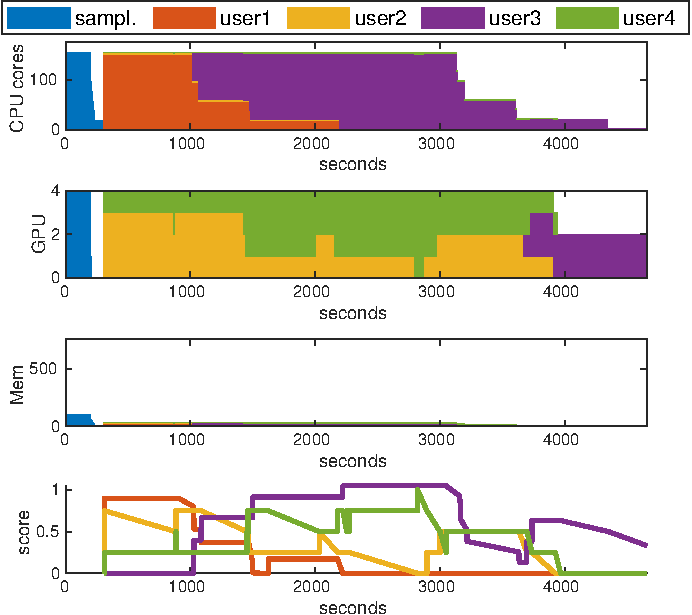
\includegraphics[width=1.0\linewidth]{figs/res_usage_allox}}
%	\caption{[Cluster] 4 users share the resource and we update fairness scores overtime to maintain the fair allocation. Sampling (sampl.) jobs are prioritized and scheduled first. \todo{fair score \& resource usage are not well synchronized as they were logged using different ways. Need to fix the plot for fairness I just saved the fairness score whenever it changes.}}
%	\label{fig:res_usage}
%\end{figure}

We first evaluate \name through real experiments and validate the accuracy of the simulator in Section~\ref{sec:eval-cluster}. Results from the simulator are discussed in Section~\ref{sec:large-sim}.
% First, we shows the improvement in terms of average completion time in \S\ref{sec:large-sim}.
% Then, we present the trade-offs between performance and fairness of \name in \S\ref{sec:tradeoffs}. 


\subsubsection{Experiments over a cluster}
\label{sec:eval-cluster}

%\paragraph{Average completion time.}
Figure \ref{fig:avgCmplt_exp} illustrates the average job completion time
under \name and other baselines through experiments and the simulator we developed. 
%\todo{Xiao \& Tan, please check the following paragraph to see if it accurately describes the insights. We need more details.}
First, Allox reduces the average completion time significantly compared to other baselines. In particular, \DRFFIFO and \DRFSJF do not fully utilize the CPU resources as shown in Figure~\ref{fig:res_util}, therefore incur longer waiting time. 
\ESRP and \DRFExt reduce the waiting time by increasing the CPU utilization (Figure \ref{fig:res_util}).
%\new{
Although \name has similar CPU and GPU utilization compared to \DRFExt and \ESRP, \name outperforms \DRFExt and \ESRP by better job scheduling and configuration selection. This is highlighted by the significant reduction in job processing time. 
%the placement of \name are more efficient than \DRFExt and \ESRP. 	
%}


%\zhenhua{Can we show the CPU/GPU utilization?} \tanle{added.}



% Although \DRFFIFO it does not suffer from the estimation overheads, the jobs are queued up on GPU and results in the worst performance.
% \DRFSJF performs much better than DRF as jobs are scheduled in the shortest job first manner.
% \ESRP is far from the optimal solution.
% Although we computed the average resource transfer rate for \DRFExt by profiling all the jobs, it does not perform well.

Figure \ref{fig:avgCmplt_exp} validates that the average completion times in the simulation and experiments are consistently similar.
This allows us to perform larger-scale evaluations using the simulator.% more extensive results without running time-consuming experiments.

\begin{figure}[t]
	\centering
%{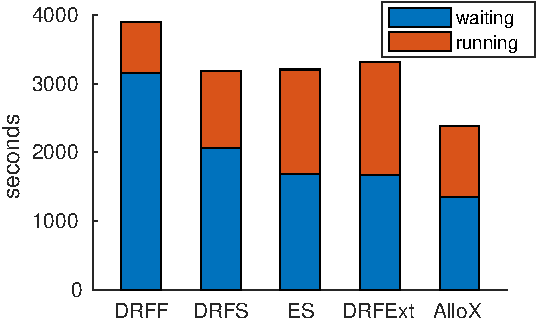
\includegraphics[width=0.7\linewidth]{figs/avgCmplt_exp}}
{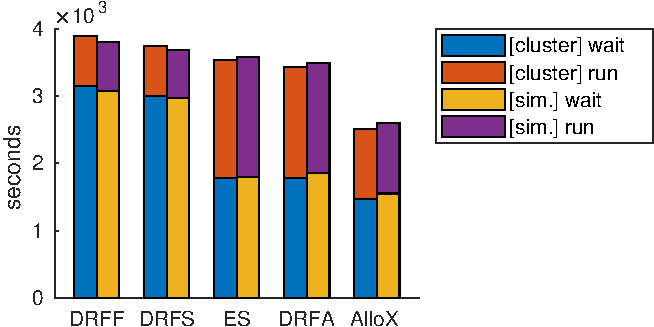
\includegraphics[width=1.0\linewidth]{figs/avg_comparison_group}}
	\caption{[Cluster] \name reduces the average job completion time. For each algorithm, the first bar shows results from experiments, and the second bar is from our simulator.} %Specifically, Allox reduces the completion time by 36\% compared to \DRFFIFO, 24\% compared to \DRFSJF, 25\% compared to \ESRP, and 27\% compared to \DRFExt. For each algorithm, the first bar shows results from experiments, and the second bar is from our simulator.} %Wrong estimation in some jobs in DRFS makes running time are longer than DRFF.}
	\label{fig:avgCmplt_exp}
\end{figure}

%\begin{figure*}[h]
%	\centering
%	\subfloat[\DRFFIFO] {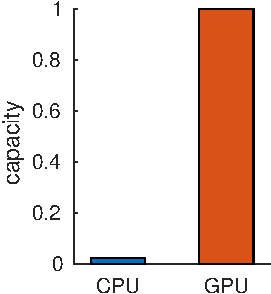
\includegraphics[width=0.15\linewidth]{figs/res_util_DRFF} \label{fig:res_util_DRFF}} 
%	\hspace{0.1cm}
%	\subfloat[\DRFSJF] {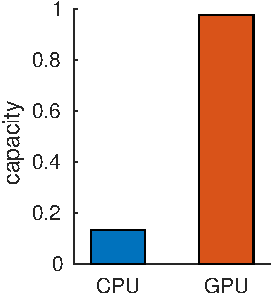
\includegraphics[width=0.15\linewidth]{figs/res_util_DRFS} \label{fig:res_util_DRFS}}  
%	\hspace{0.1cm}
%	\subfloat[\ESRP] {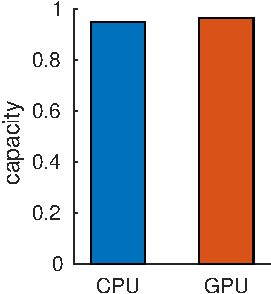
\includegraphics[width=0.15\linewidth]{figs/res_util_ES} \label{fig:res_util_ES}} 
%	\hspace{0.1cm} 
%	\subfloat[\DRFExt] {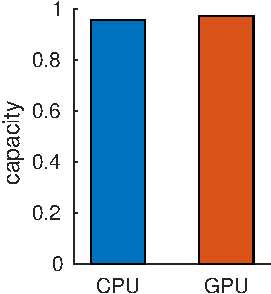
\includegraphics[width=0.15\linewidth]{figs/res_util_DRFExt} \label{fig:res_util_DRFExt}}  
%	\hspace{0.1cm}
%	\subfloat[\name] {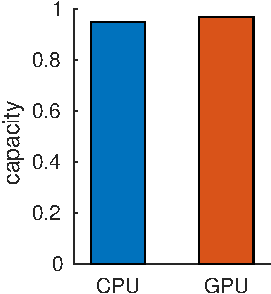
\includegraphics[width=0.15\linewidth]{figs/res_util_AlloX} \label{fig:res_util_AlloX}}     
%	\caption{[Cluster] Resource Utilization.}
%	\label{fig:res_util}
%\end{figure*}

\begin{figure}[b]
	\centering
	 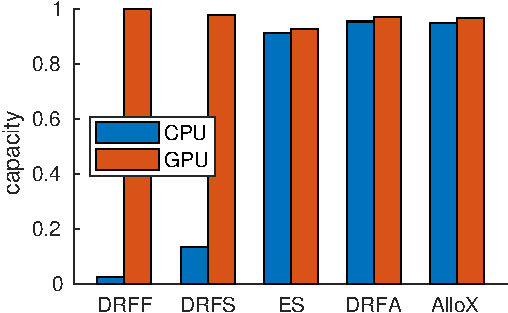
\includegraphics[width=0.7\linewidth]{figs/res_util}  
	\caption{[Cluster] CPU and CPU utilization.}
	\label{fig:res_util}
\end{figure}

%\begin{figure}[H]
%	\centering
%{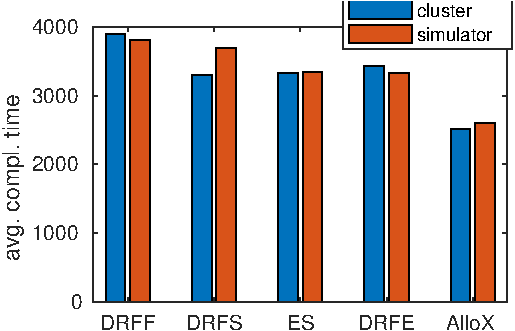
\includegraphics[width=0.7\linewidth]{figs/avg_comparison}}
%	\caption{[Cluster] vs [Simulator]}
%	\label{fig:avgCmplt_exp}
%\end{figure}
